\textbf{Autor: Tugce}\\
\begin{figure}[ht]
	\centering
  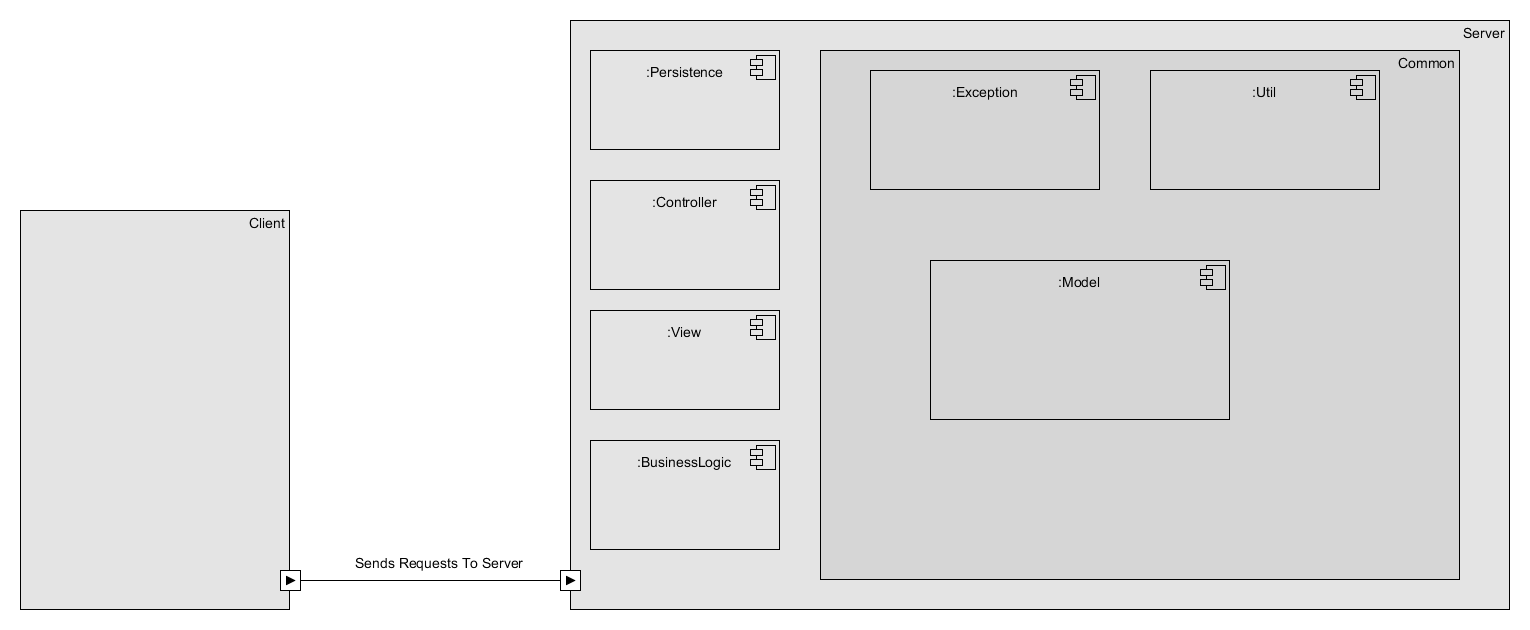
\includegraphics[width=\textwidth,height=15cm,keepaspectratio]{../UMLDiagramme/A-Sicht}
	\caption{Konzeptionelle Sicht - Komponentendiagramm}
	\label{fig15}
\end{figure}
Die Abbildung \ref{fig15} zeigt das Laufzeitverhalten des Systems.\\
Die Interaktion mit dem Softwaresystem erfolgt über eine klassische Client-Server-Struktur.  Es gibt einen Server und beliebig viele Clients, die mit dem Server interagieren. Der Server beinhaltet alle Komponenten des Softwaresystems und der Server verarbeitet die Requests der Clients.   \\
Der Benutzer greift über seinen Browser (Client) auf die Website zu. Die angesteuerte Website ist die index.xhtml. Dabei erhält der Nutzer eine eigene Session. Auf der index.xhtml kann sich der Nutzer einloggen und weitere Teile des Softwaresystems erreichen.
Die Ausführungssicht beinhaltet alle in den vorherigen Sichten getroffenen Entscheidungen. Daher gibt es die aufgeführten Pakete in der Abbildung \ref{fig15} (Common, Persistence, View, Controller). Dadurch das es keine seperate App für mobile Geräte gibt, ist das Ausführungsverhalten auf allen Geräten gleich. Durch die in der Modulsicht getroffene Entscheidung Daten-Backups anzulegen, werden auf dem Server Backup-Dateien abgelegt. Die Datenbank für das Softwaresystem ist ebenfalls auf dem Server. 